\chapter{Introduction}
\label{sec:intro}
\section{Solving Equations}
Solving systems of polynomial equations is a core goal of mathematics. Algebraic geometry is the subfield of mathematics concerned with describing the geometry of set of solutions to such systems of equations. A typical first step is to establish some qualitative facts about the space of solutions, for example to check whether it is nonempty, and if so, find its dimension.

 After establishing that solutions to a given system of polynomial equations exist, a natural question is whether the solutions can be written in an explicit, parametric form. Ideally, such a parametrization should be by simple functions defined on a simple domain. For systems of linear equations, the solution set can always be parametrized by linear functions defined on affine space. When we consider systems of polynomial equations instead, we want to parametrize the solutions by polynomial functions on affine space, or more generally by quotients of such polynomials.

A classic example of such a parametrization is stereographic projection. The points on the unit sphere are the solutions to the equation
\begin{equation}
	\label{eq:Stereographic1}
	x^2 + y^2 + z^2 = 1.
\end{equation}
Since the solution set is two-dimensional, we want to parametrize it by two free parameters $u,v$. We can do this as follows:
\begin{equation}
	\label{eq:Stereographic2}
	(x,y,z) = \left(\frac{2u}{1+u^2+v^2}, \frac{2v}{1+u^2+v^2}, \frac{-1+u^2+v^2}{1+u^2+v^2} \right).
\end{equation}

We can understand the parametrization geometrically, see \cref{fig:StereographicProjection}. Consider the line connecting a point $(u,v)$ in the $(x,y)$-plane with the point $P = (0,0,1)$. Map $(u,v)$ to the unique point $(x,y,z)$ on this line, different from $P$, such that $(x,y,z)$ solves \eqref{eq:Stereographic1}.
This parametrization describes all solutions to \eqref{eq:Stereographic1}, except the point $P$ itself.
\begin{figure}
	\centering
	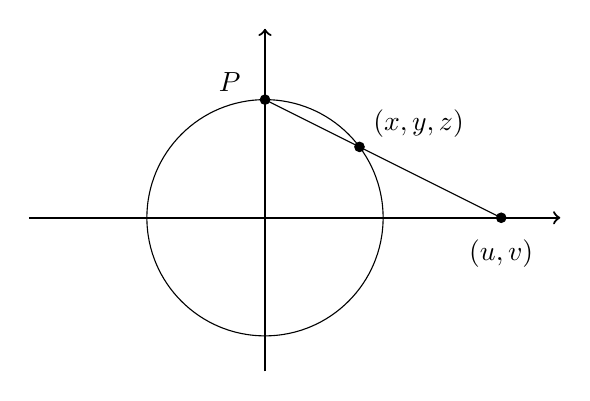
\begin{tikzpicture}[scale = 1.5]
		\draw[thick, ->] (-2,0) -> (2.5,0);
		\draw[thick, ->] (0,-1.3) -> (0,1.6);
		\draw (0,1) -> (2,0);
		\draw (0,0) circle (1);
		\draw[fill] (0,1) circle (0.04);
		\node at (-0.3,1.15) {$P$};
		\draw[fill] (0.8,0.6) circle (0.04);
		\node at (1.3,0.8) {$(x,y,z)$};
		\draw[fill] (2,0) circle (0.04);
		\node at (2,-0.3) {$(u,v)$};
	\end{tikzpicture}
	\caption{A two dimensional slice of a stereographic projection}
	\label{fig:StereographicProjection}
\end{figure}

In contrast to the linear case, admitting such a parametrization is a very restrictive condition on a system of polynomial equations. Rationality questions are concerned with studying when such a parametrization exists. 

There are also many interesting notions of being ``close to'' parametrizable by affine space. Contributing to the study of how these notions relate to each other, and how one can prove the nonexistence of such a parametrization, is an overarching goal of this thesis. As we will see, tools from many branches of mathematics can be applied to rationality questions. Algebraic tools are of course crucial to any work in algebraic geometry, but since we will primarily work over the complex numbers, we will also draw on ideas from topology and differential geometry.

\section{The Rationality Hierarchy}
To formalize the discussion above, we introduce some basic concepts from birational geometry. Let $X$ and $Y$ be varieties over a field $k$. A rational map $f \from X \ratmap Y$ is a morphism $f \from U \to Y$, where $U \subset X$ is a nonempty open set. The rational map $f \from X \ratmap Y$ is a birational map, written $f \from X \birat Y$, if there is a rational map $g \from Y \ratmap X$, such that both $g \circ f$ and $f \circ g$ are the identity map on an open set where both maps are defined.

We call a variety rational if it is parametrizable in the following sense.
\begin{definition}
	\label{def:Rational}
	A variety $X$ over a field $k$ of dimension $n$ is \emph{rational} if there exists a birational map $f \from \P^n \birat X$. Equivalently, the function field $k(X)$ is a purely transcendental extension of $k$.
\end{definition}
Affine space is an open dense subset of $\P^n$, so a rational variety is also parametrized almost everywhere by affine space. However, it is more convenient to work with projective space.

To describe varieties that are not rational, we will use the terms \emph{irrational} and \emph{nonrational} interchangeably.

Recall that a rational map $f \from X \ratmap Y$ is \emph{dominant} if its image is dense. A weaker version of being parametrizable by $\P^n$ is the following.
\begin{definition}
	\label{def:Unirational}
	Let $k$ be a field of characteristic 0. A variety $X$ over a field $k$ of dimension $n$ is \emph{unirational} if there exists a dominant rational map $f \from \P^m \ratmap X$. Equivalently, the function field $k(X)$ is a subfield of a purely transcendental extension of $k$.
\end{definition}
\begin{remark}
	If any such dominant map $f$ exists, and the field $k$ is infinite, then one may assume that $f$ is a generically finite morphism by restricting $f$ to a general linear subspace $\P^n \subset \P^m$ of suitable dimension.
\end{remark}
Starting from these two classical properties, a hierarchy of rationality properties has been studied, each capturing different notions of when a variety $X$ is close to being rational. We collect and motivate three important such properties here.
\begin{definition}
	\label{def:StablyRational}
	A variety $X$ is \emph{stably rational} if $X \times \P^m$ is rational for some $m$. Equivalently, there exists a purely transcendental extension $k(X)(t_1,\dots,t_m)$ of $k(X)$, such that this extension is a purely transcendental extension of $k$.
\end{definition}
Stable rationality traces its roots back to the following question by Zariski.
\begin{question}[Zariski problem]
	\label{que:Zariski}
	Let $K$ and $K'$ be finitely generated fields over a field $k$ such that there exists simple transcendental extensions of $K$ and $K'$ that are isomorphic. Must then $K$ and $K'$ be isomorphic?
\end{question}
For many varieties, including many natural moduli spaces (see \eg \cite{Ballico}, \cite{KollarSchreyer}), it is possible to check that they are stably rational, while the question of rationality remains open.

There is also an associated equivalence relation, where we say that two varieties, $X,Y$, are \emph{stably birational}, or \emph{stably birationally equivalent}, if $X \times \P^n \birat Y \times \P^m$ for some $n,m$. We say that an invariant associated to a variety $X$ is a \emph{stable birational invariant} if it is preserved by stable birational equivalence.

\begin{definition}
	\label{def:RetractRational}
	A variety $X$ is \emph{retract rational} if there are rational maps $f \from X \ratmap \P^N$ and $g \from \P^N \ratmap X$ and an open subset $U \subset X$, such that $g \circ f$ is defined on $U$ and $g \circ f \from U \to U$ is the identity.
\end{definition}
The definition of retract rationality is the hardest one to motivate. It was originally introduced in an algebraic context by Saltman in \cite{SaltmanHomage}, with a goal of understanding how rationality relates to certain approximation properties. More geometrically, a natural question arising from the definition of stable rationality is whether a stably irrational variety $X$ could be a factor in a rational variety. It is not hard to see that if $X \times Y$ is rational for some variety $Y$, then $X$ is retract rational, so studying retract rationality can answer this question. Finally, retract rationality is interesting because of its relation to decompositions of the diagonal, see \cref{prop:RetractRationalDecomposition}. This makes it the natural rationality property to investigate with this powerful tool.

The final rationality property we introduce is rational connectedness.
\begin{definition}
	\label{def:RationallyConnected}
	A variety $X$ over an uncountable algebraically closed field $k$ is \emph{rationally connected} if for any two general points $y,x \subset X$ there is a map $\P^1_k \to X$, defined over $k$, such that $0 \mapsto x$ and $\infty \mapsto y$.
\end{definition}
Rational connectedness is a relatively weak property, but it is well-behaved and usually easy to check. For example, one can prove that in a family of smooth varieties, if the generic member is rationally connected, then every member is rationally connected. The corresponding statement for \eg unirationality is not known. Furthermore, if a smooth variety contains a rational curve with ample normal bundle, it is rationally connected, and in characteristic 0 a smooth Fano variety is rationally connected. Proofs of these statements can be found in \cite[IV.3, V.2]{KollarRationalCurves}.

We have the following straightforward implications between the five rationality properties we have introduced.
\begin{proposition}
	\label{prop:RationalityHierarchy}
	Let $X$ be a variety over a field $k$. Then each property in this list implies the next. %\todo{Add nice arrows?}
	\begin{enumerate}[i)]
		\item $X$ is rational.
		\item $X$ is stably rational.
		\item $X$ is retract rational.
		\item $X$ is unirational.
		\item $X$ is rationally connected.
	\end{enumerate}
\end{proposition}
Studying when, if at all, the converse implications hold, has been a major and fruitful area of birational geometry. For curves, clearly rationally connected implies unirational. Furthermore, by Lüroth's theorem, all five properties coincide.
\begin{theorem}[{Lüroth's theorem (\cite[Example 2.55]{Hartshorne})}] %\todo{Should I reference the original, or maybe not at all?}
	\label{thm:Lueroth}
	Let $k$ be a field, $t$ a transcendental element over $k$, and $k(t)/K/k$ field extensions. Then $K$ is also a purely transcendental extension of $k$.
\end{theorem}
In geometric language, \cref{thm:Lueroth} states that any unirational curve is rational. To see this geometric implication, assume that $X$ is a curve and $f \from \P^1 \ratmap X$ is a rational map. Then we have the following tower of field extensions: $k(t)/k(X)/k$. By \cref{thm:Lueroth}, $k(X)$ must be a purely transcendental extension of $k$ of degree $1$, hence $k(X) \simeq k(t)$. So the curve $X$ must be rational. Because of this result, studying the relationship between unirationality and rationality has been known as the \emph{Lüroth problem}.

A major achievement of the Italian school of algebraic geometry is the proof that for smooth surfaces over an algebraically closed field of characteristic 0, the five properties in \cref{prop:RationalityHierarchy} are also equivalent. To see this, one first checks that if $X$ is rationally connected, then there is a dominant map $f \from C \times \P^1 \ratmap X$ for some curve $C$. This implies that all plurigenera of $X$ are zero, so $X$ is rational by Castelnuovo's criterion for rationality (\cite[V.6.2]{Hartshorne}). In positive characteristic however, unirational surfaces that are not rational exist. Examples of this were found by Zariski (see \cite{Zariski58}).

Starting from dimension 3, the properties in \cref{prop:RationalityHierarchy} are no longer equivalent, even over $\C$. Already in the early twentieth century Fano claimed to have found an example of a unirational, non rational threefold. However, the proof contained gaps.
%have a proof that the intersection of a quadric and a cubic hypersurface in $\P^5$, which is a unirational variety, is not rational. However the proof contained gaps. Later, Roth claimed to construct a complex unirational variety which was not simply connected, and hence not rational. However, also this proof contained errors, and  Serre later proved that any complex unirational variety is simply connected. %\todo{Keep this historical note?}
Thus, the answer would first come in the early 1970s; three examples appeared independently of irrational, unirational threefolds.

First, following the original ideas of Fano, Iskovskikh and Manin proved
in \cite{IskovskikhManin}
that any birational automorphism of a smooth quartic threefold is in fact biregular. On the other hand, $\P^3$ has infinitely many birational, but not biregular, automorphisms. Therefore, a smooth quartic threefold cannot be rational.
%the following.
% \begin{theorem}[{\cite{IskovskikhManin}}]
	% 	\label{thm:QuarticRigidity}
	% 	Let $X \subset \P^4$ be a smooth quartic threefold, then any birational automorphism of $X$ is in fact a biregular automorphism. In particular, $X$ is not rational.
	% \end{theorem}
% The implication that $X$ is irrational follows since $\P^n$ has infinitely many birational, but not biregular, automorphisms.
In \cite{SegreVariazioneContinua}, Segre had constructed a smooth, unirational quartic hypersurface, so this gave the first counterexample to the Lüroth problem.

Around the same time, Clemens and Griffiths introduced
in \cite{ClemensGriffiths}
a rationality criterion based on the intermediate Jacobian and used it to prove that no smooth cubic threefold is rational.
% the following rationality criterion.
% \begin{theorem}[{\cite{ClemensGriffiths}}]
	% 	Let $X$ be a smooth rational threefold. Then its intermediate Jacobian is the product of Jacobians of curves.
	% \end{theorem}
% They also apply the criterion to cubic threefolds.
% \begin{theorem}[{\cite{ClemensGriffiths}}]
	% 	\label{thm:CubicThreefoldIrrational}
	% 	The intermediate Jacobian of a smooth cubic threefold is not a product of Jacobians of curves, and therefore irrational.
	% \end{theorem}
Projecting from any line in a cubic threefold gives the threefold a conic bundle structure, hence a smooth cubic threefold is unirational. These examples prove that even over $\C$, the properties in \cref{prop:RationalityHierarchy} are no longer equivalent,  starting from dimension 3.

However, the obstructions to rationality used by
Iskovskikh-Manin and Clemens-Griffiths
only obstruct rationality, and not the weaker properties in \cref{prop:RationalityHierarchy}. So more examples are necessary to understand the relation between the various other rationality properties.

Shortly after the work of Iskovskikh-Manin and of Clemens-Griffiths appeared, Artin and Mumford constructed one such example.
\begin{theorem}[{\cite{ArtinMumford}}]
	\label{thm:ArtinMumfordIntroduction}
	There exists a unirational double cover $X \to \P^3$, admitting a desingularization $\widetilde{X} \to X$, such that $H^3(\widetilde{X},\Z)$ has nontrivial torsion. Since this torsion group is a stable birational invariant of smooth complex varieties, $\widetilde{X}$ is not stably rational.
\end{theorem}
We will soon see that this invariant proves that $X$ has no decomposition of the diagonal, and is therefore also not retract rational. Although these concepts were not introduced at the time of \cite{ArtinMumford}, \cref{thm:ArtinMumfordIntroduction} also proves that retract rationality is a stronger property than unirationality.

Regarding the relation between rationality and stable rationality, Beauville, Colliot-Thélène, Sansuc and Swinnerton-Dyer answered \cref{que:Zariski} negatively over $\C$. In the paper \cite{BCTSSD} they find a smooth, irrational, complex threefold $X$ such that $X \times \P^3$ is rational. In fact, Shepherd-Barron proves in \cite{Shepherd-Barron} that also $X \times \P^2$ is rational. As far as the author is aware, this is essentially the only known example of an irrational, but stably rational, complex variety.

These examples prove that most of the implications in \cref{prop:RationalityHierarchy} are not equivalences. The following two questions remain.
\begin{question}
	\label{que:StableVsRetract}
	Does there exist a retract rational variety that is not stably rational?
\end{question}

\begin{question}
	\label{que:RationallyConnectedVsUnirational}
	Does there exist a rationally connected variety that is not unirational?
\end{question}
Especially the latter question is a major open problem in birational geometry. The answer to both of these questions is widely expected to be positive, but constructing examples illustrating this has proven to be difficult.

\section{Retract Rationality and Unirationality of Certain Complete Intersections}
The papers in the thesis fall into two categories. The three first papers fall into the first category, namely studying rationality properties of certain simple varieties. The thesis begins with two papers proving retract irrationality of two complete intersections in projective space. The third paper studies unirationality of double covers and complete intersections of quadrics.

\subsection{Specialization and Decomposition of the Diagonal}
% A large part of the difficulty in distinguishing the properties in \cref{prop:RationalityHierarchy}, lies in finding invariants that obstruct some, but not all of the properties. So for any (stably) birational invariant, it is an interesting question if it can be nontrivial on rationally connected varieties.

%In this thesis, we will focus on other invariants, which are potentially useful in higher dimensions. We will focus on understanding these invariants on so-called Fano varieties. Recall that a variety $X$ is called a \emph{Fano variety} if the anticanonical divisor $-K_X$ is ample. It is a celebrated result by Mori that in characteristic 0, any Fano variety is rationally connected. In particular, we will concentrate on some central examples of Fano varieties, hypersurfaces, complete intersections and double covers. The space of rational curves on a Fano variety $X$ contains much information about the geometry of $X$. And in the later sections of the thesis, we focus on birational invariants related to curves on $X$, and how studying the space of rational curves lets us compute these invariants. \todo{Maybe this general principle should be emphasized more?}
We first introduce the concept of a \emph{decomposition of the diagonal}. This plays the main role in \cref{pap:23diagonal} and \cref{pap:33diagonal}. It also has strong implications for all the the other rationality properties and birational invariants we study throughout the thesis. Decomposition of the diagonal with rational coefficients were introduced in by Bloch and Srinivas in \cite{BSCorrespondences}. Beginning with Voisin's landmark paper \cite{VoisinDoubleQuartic}, its relation to rationality properties has attracted much attention.
\begin{definition}
	\label{def:DoD}
	Let $X$ be a scheme of pure dimension $n$. We say that $X$ admits a (Chow theoretic) \emph{decomposition of the diagonal} if the following equality holds in $\CH_n(X \times X)$, with coefficients in $\Z$,
	\begin{equation}
		\label{eq:DefinitionDoD}
		[\Delta_X] = [X \times z] + [W].
	\end{equation}
	Here $z \in X$ is a zero cycle of degree 1 and $W$ is supported on $D \times X$, with $D \subsetneq X$ a closed subscheme of $X$.
\end{definition}
If \eqref{eq:DefinitionDoD} holds in $\CH(X \times X) \otimes \Q$ instead, we say that $X$ admits a \emph{decomposition of the diagonal with rational coefficients}.
%If such an equality holds in the cohomology ring $H^*(X \times X,\Z)$ instead, we say that $X$ admits a cohomological decomposition of the diagonal.

% For proper varieties there is also the following alternative viewpoint.
% \begin{definition}
% 	Let $X$ be a proper variety over a field $k$. We say that the Chow group of zero-cycles $\CH_0(X)$ is \emph{universally trivial} if for any field extension $K/k$, the degree map $\deg \from \CH_0(X_K) \to \Z$ is an isomorphism.
% \end{definition}
% \begin{proposition}[{\cite[Proposition 1.4]{ColliotThelenePirutka}}]
% 	\label{prop:DecompositionCH0Trivial}
% 	A smooth, proper, geometrically integral variety $X$ has a decomposition of the diagonal if and only if $\CH_0(X)$ is universally trivial.
% \end{proposition}

A decomposition of the diagonal is closely related to three of the properties in \cref{prop:RationalityHierarchy}. We summarize this connection with three results. For proofs and references to the papers where these concepts and results first appeared, see Schreieder's excellent survey \cite{SchreiederCyclesAndRationality}.
\begin{proposition}[{\cite[Section 7.2]{SchreiederCyclesAndRationality}}]
	If a variety $X$ is rationally connected, then there exists an integer $N$, such that $N[\Delta_X]$ has a decomposition as in \eqref{eq:DefinitionDoD}.
\end{proposition}
%
%\begin{definition}
%	For a proper variety $X$, the smallest positive integer $N$ such that $N[\Delta_X]$ admits a decomposition of the diagonal, is known as the \emph{torsion order}, and is a stable birational invariant of smooth varieties.
%\end{definition}

\begin{proposition}[{\cite[Corollary 7.12]{SchreiederCyclesAndRationality}}]
	If there is a dominant map $\P^n \ratmap X$ of degree $N$ \ie $X$ has a unirational parametrization of degree $N$, then $N[\Delta_X]$ has a decomposition as in \eqref{eq:DefinitionDoD}.
\end{proposition}
%Mention that this $N$ is called the torsion order

\begin{proposition}[{\cite[Lemma 7.4]{SchreiederCyclesAndRationality}}]
	\label{prop:RetractRationalDecomposition}
	If $X$ is retract rational, then $X$ has a decomposition of the diagonal.
\end{proposition}

Also, if a variety $X$ admits a decomposition of the diagonal, this forces many birational invariants to be trivial. We illustrate the principle with the following result and proof.
\begin{proposition}[{\cite[Theorem 3.4]{VoisinAbelJacobi}}]
	\label{thm:DecompositionAndH3}
	Let $X$ be a complex threefold admitting a decomposition of the diagonal, then $H^3(X,\Z)$ has no torsion.
\end{proposition}
\begin{proof}
	If we think of both sides of \eqref{eq:DefinitionDoD} as representing self-correspondences of $X$, they both act on $H^3(X,\Z)$. The left hand side acts as the identity, and the action of the right hand sides takes classes in $H^3(X,\Z)$ to classes in $H^1(\widetilde{W},\Z)$, for some desingularization $\widetilde{W}$ of $W$. This cannot have any torsion. Hence, the image of the identity map on $H^3(X,\Z)$ has no torsion.
\end{proof}
This proves that the variety $\widetilde{X}$ from \cref{thm:ArtinMumfordIntroduction} does not admit a decomposition of the diagonal. Hence, by \cref{prop:RetractRationalDecomposition}, it is not retract rational.

\begin{remark}
	There are smooth, irrational varieties that admit a decomposition of the diagonal (see \cite{ColliotThelenePresqueDiagonales}), but it is an open question if there are smooth, non retract rational varieties with a decomposition of the diagonal.
\end{remark}

We can now set the stage for the first two papers in this thesis. Starting with Koll\'ar's paper \cite{KollarHypersurfaces}, specialization methods have been used to study rationality questions. The basic idea is that we can prove irrationality of a given variety $X$ by finding a reference variety $X_0$ with some nontrivial birational invariant and a specialization of $X$ to $X_0$ that preserves this birational invariant.

There are three main such specialization methods, detecting increasingly strong rationality properties. The method from \cite{KollarHypersurfaces} is based on ruledness (being birational to a product $Y \times \P^1$). The important point is that ruledness is preserved under specialization. For complex hypersurfaces of sufficiently large degree, Koll\'ar constructs a specialization to a variety in positive characteristic that admits a global differential form. This special variety can therefore not be ruled, and hence the general fiber is likewise not ruled. With this strategy, Koll\'ar proves that a very general complex hypersurface in $\P^{n+1}$ of degree $\frac{2}{3}(n+3)$ is not ruled, and hence not (stably/retract) rational.

A breaktrough in specialization methods was introduced by Voisin in \cite{VoisinDoubleQuartic}. The important point is that having a decomposition of the diagonal is preserved under specialization, as long as the special fiber satisfies certain smoothness conditions. This is in contrast to many other birational invariants, such as torsion in $H^3(X,\Z)$. By specializing a very general double quartic solid to the example of Artin and Mumford, Voisin proves that the special fiber cannot have a decomposition of the diagonal. Hence, the very general fiber cannot have a decomposition of the diagonal, and is therefore retract irrational.

This specialization technique was then developed further by Colliot-Thélène and Pirutka in \cite{ColliotThelenePirutka} and by Schreieder in \cite{SchreiederHypersurface}, proving retract irrationality of a very general quartic threefold, and hypersurfaces in $\P^{n+1}$ of degree at least $\log_2 n + 2$, respectively.

The final specialization method relevant here is based on the motivic volume introduced by Nicaise and Shinder in \cite{NicaiseShinderMotivic}. This was developed further by Kontsevich and Tschinkel in \cite{KontsevichTschinkelSpecialization} and by Nicaise and Ottem in \cite{NicaiseOttemRefinement}. The motivic volume was used by Nicaise and Ottem in \cite{NicaiseOttem} to prove stable irrationality of many complete intersections whose irrationality was previously unknown.

The specialization method is based on the ring of stable birational types; equivalence classes under stable birational equivalence. In this ring, the sum and product are induced by disjoint unions and Cartesian products, respectively. If a specialization of a variety over a field of characteristic 0 is not too singular, there is a ring homomorphism taking the stable birational type of the generic fiber to the stable birational type of the special fiber. So if the stable birational type of the special fiber is nontrivial, the stable birational type of the generic fiber must be nontrivial as well. Because of the ring structure, this technique is particularly well suited to specializing to fibers with multiple components.

The specialization methods outlined above are powerful, but they all require as input some example where irrationality can be verified in another way. For this, other birational invariants are required. One such invariant is the unramified cohomology group $H_{nr}^2(k(X)/k,\mu_2^{\otimes 2})$. This stable birational invariant is closely related to torsion in $H^3(X,\Z)$ (c.f. \cref{thm:ArtinMumfordIntroduction}). In fact, for smooth varieties this particular unramified cohomology group is isomorphic to the cohomological Brauer group, which in turn is isomorphic to torsion in $H^3(X,\Z)$. A reason to use this particular birational invariant is the remarkable example found by Hassett, Pirutka and Tschinkel in \cite{HPTActa} of a quadric surface bundle $X \to \P^2$ with nontrivial unramified cohomology. This quadric surface bundle has proven to be a very useful target for specializations.

\subsection{Summary of \cref{pap:23diagonal}}
The three specialization techniques outlined above preserve different rationality properties. So comparing the three techniques can potentially shed light on how the corresponding rationality properties can differ. In light of the question of whether stable and retract rationality are equivalent (\cref{que:StableVsRetract}), it is particularly interesting if the specialization method based on decomposition of the diagonal is applicable to the examples where stable rationality was first proven in \cite{NicaiseOttem}. One such example is the complete intersection of a quadric and a cubic hypersurface in $\P^6$.

In \cref{pap:23diagonal}, we use the specialization technique based on decomposition of the diagonal to prove that the very general intersection of a quadric and a cubic hypersurface in $\P^6$ is not retract rational. With this result, the cubic fourfold is the only complete intersection in dimension 4
for which retract rationality of a very general member remains open.

 An additional goal of \cref{pap:23diagonal} is to find explicit examples of retract irrational complete intersections, complementing the result about the very general intersection. Specifically, we find examples defined over countable fields, such as $\Q$, of non retract rational complete intersections of a quadric and cubic hypersurface in $\P^6$. To find examples over countable fields, it is necessary to specialize to positive characteristic.

The main result of the paper is.
\begin{theorem}
	\label{thm:SpecializationIntroduction}
	Let $K=\Q$ or $K=\F_p(t)$ with $p \geq 3$. In the first case let $p \geq 3$, $q \geq 11$ be distinct primes and set $u=p,v=q$, and in the second case let $u=t,v=(t-1)$. Let $X \subset \P^6_K$ be the complete intersection defined by the following two equations:
	\begin{equation}
		\ u \left(\sum_{i=0}^6 x_i^2 \right) + v(x_3x_6-x_4x_5)=0
	\end{equation}
	
	\begin{align}
		u \left(\sum_{i=0}^6 x_i^3 \right) + v(x_0^2x_5 &+ x_1^2x_4 + x_2^2x_6 \nonumber \\
		 &+ x_3(x_5^2+x_4^2+x_3^2 -2x_3(x_6 + x_5 + x_4)))=0.
	\end{align}
	Then $X$ is a smooth complete intersection such that the base change to $\overline{K}$ does not admit a decomposition of the diagonal. It is therefore not geometrically retract rational.
\end{theorem}
\begin{remark}
	Since the complete intersection $X$ in \cref{thm:SpecializationIntroduction} is smooth, it is straightforward to use a second specialization argument to prove that the very general complete intersection of a cubic and quadric hypersurface in $\P^6$ over $\C$ is not retract rational.
\end{remark}
We prove \cref{thm:SpecializationIntroduction} using a specialization heavily inspired by the one used in \cite{NicaiseOttem}. The complete intersection is specialized to a complete intersection singular along a plane. After blowing up the plane, one obtains a variety birational to the quadric surface bundle from \cite{HPTActa}. The exceptional locus of the blowup is a rational quadric bundle. To obstruct the existence of a decomposition of the diagonal on this union we rely heavily on the techniques in \cite{SchreiederHypersurface}. The main point is identifying a nontrivial unramified cohomology class on the blowup, namely the one found in \cite{HPTActa}. This nontrivial class obstructs a decomposition of the diagonal on the special fiber. The main innovation in \cref{pap:23diagonal} lies in using the unramified cohomology class on the blowup of the special fiber to prove that the special fiber itself does not admit a decomposition of the diagonal. Additionally, there is some work involved in picking the exact equations and verifying the technical details for this particular choice.

\subsection{The Specialization Technique of Pavic and Schreieder}
The specialization method in \cref{pap:23diagonal} is also applicable when specializing to a union of two varieties. However, it is crucial that the obstruction to rationality lies on one of the components of the special fiber. The intersection of the components must be rational, or at least the obstruction to rationality should vanish on the intersection.

Contrast this with the method in \cite{NicaiseOttem}, which also works well when specializing such that two rational components meet in a stably irrational locus. In fact, such specializations often give the most powerful results. Especially in higher dimensions, this flexibility lets one prove stable irrationality of many complete intersections. By specializing to a union whose intersection is stably irrational, Nicaise and Ottem prove that for the following four complex fivefolds, the very general such fivefold is stably irrational: the quartic fivefold, the intersection of two cubics in $\P^7$, the intersection of two quadrics and a cubic in $\P^8$ and finally the intersection of four quadrics in $\P^9$.

Since the specialization method of Nicaise and Ottem does not say anything about retract rationality, studying retract rationality of these fivefolds is an interesting problem. With this in mind, Pavic and Schreieder develop in \cite{PavicSchreieder} a new obstruction to the existence of a decomposition of the diagonal. This obstruction is suitable for specializations to a union where the intersection does not admit a decomposition of the diagonal. Working with this obstructions is quite technical, but very broadly, the main idea is to study the $\CH_1$ group of the special fiber.
%The nature of the obstruction is summarized well by the following result.
%\begin{theorem}[{\cite[Corollary 1.3]{PavicSchreieder}}]
%	\label{thm:PSCorollaryIntro}
%	Let $R$ be a DVR with algebraically closed residue field $k$ and let $\pi \from \mathcal{X} \to \Spec R$ be a projective semi-stable $R$-scheme whose special fiber $Y = Y_1 \cup Y_2$ has two components. Assume that
%	\begin{itemize}
%		\item $Y$ is universally $\CH_1$-trivial in the sense that for any field extension $L/k$, the natural map $\CH_1(Y) \to \CH_1(Y_L)$ is surjective;
%		\item $Y_{12} \coloneqq Y_1 \cap Y_2$ is integral and its torsion order is even.
%	\end{itemize}
%	Then the geometric generic fiber of $\pi$ does not admit a decomposition of the diagonal.
%\end{theorem}
In \cite{PavicSchreieder}, Pavic and Schreieder also apply this obstruction to prove that over an algebraically closed field of characteristic different from $2$, the very general quartic fivefold does not admit a decomposition of the diagonal, and is therefore not retract rational.

\subsection{Summary of \cref{pap:33diagonal}}
Comparing the obstructions in \cite{NicaiseOttem} and \cite{PavicSchreieder} is a very interesting question, since they detect different kinds of rationality and are, at least a priori, unrelated. A natural starting point is to check if the techniques in \cite{PavicSchreieder} suffice to prove retract irrationality of the fivefolds whose stable irrationality was first proven in \cite{NicaiseOttem}. The goal of \cref{pap:33diagonal} is to take a step in this direction by applying the method of \cite{PavicSchreieder} to the very general intersection of two cubics in $\P^7$.

The core idea in the specialization is the same as in \cite[Theorem 7.2]{NicaiseOttem}. By specializing one of the cubics to the union of a hyperplane and a quadric, the special fiber is a union of two components meeting along the intersection of a quadric and a cubic in $\P^6$. From \cref{pap:23diagonal}, we know this variety is not retract rational. After setting up this specialization, a technical section follows where we check that the obstruction from \cite{PavicSchreieder} can be applied, which proves that the very general intersection of two cubic sixfolds does not admit a decomposition of the diagonal.

The technical work consists of two specializations. First we modify a naïve specialization to a union of two components through a series of blowups, such that the obstruction of Pavic and Schreieder applied. In a second part, we further specialize the special fiber to better control $\CH_1$ of the two components. The main tool is specializing such that the components become rational, which simplifies $\CH_1$. Throughout we follow the argument in \cite{PavicSchreieder} very closely. The main novel contribution of \cref{pap:33diagonal} lies in finding a concrete specialization of an intersection of two cubic sixfolds, and further showing how we can simplify $\CH_1$ to apply the obstruction from \cite{PavicSchreieder}. We obtain the following theorem:
\begin{theorem}
	Let $k$ be an uncountable algebraically closed field of characteristic $0$. Then the very general complete intersection of two cubic hypersurfaces in $\P^7_k$ does not admit a decomposition of the diagonal, and is therefore not retract rational.
\end{theorem}
In this paper, we only work over characteristic $0$ to keep the proofs slightly less technically demanding. But, as is explained in \cref{pap:33diagonal}, only small modifications of the proof are necessary to prove the main result over an algebraically closed field of characteristic different from $2$ and $3$.

\subsection{Unirationality in High Dimensions}
We next turn our attention to unirationality. Here we also first encounter double covers of projective space. This is another classical construction of algebraic varieties and will play an important role in the remainder of the thesis.

Let $X$ be a hypersurface, a complete intersection or a double cover. It is natural to ask how the rationality properties of $X$ depend on the degree and dimension of $X$. In one direction, we want a lower bound on the degree, depending on the dimension of $X$, such that if the degree of $X$ exceeds this bound, a general $X$ does not have a given rationality property. In this direction, Schreieder has found a logarithmic bound on the degree of hypersurfaces, such that the very general hypersurface of degree exceeding this bound is not retract rational (\cite{SchreiederHypersurface}). For double covers, or more generally cyclic covers, the same question has been studied by Okada in \cite{OkadaCyclicCovers} and by Schreieder in \cite[Theorem 9.1]{SchreiederHypersurface}.

%  Okada proves in \cite[Theorem 1.1]{OkadaCyclicCovers} that a very general cyclic cover $p \from X \to \P^n$ of dimension $n \geq 3$ and branched along a hypersurface of degree $d \geq n+1$, is not stably rational. Schreieder remarks in \cite{SchreiederHypersurface} that the techniques developed in that paper give the following result for double covers.
% \begin{theorem}[{\cite[Theorem 9.1]{SchreiederHypersurface}}]
	%   Let $N \geq 3$ be a positive integer, and write $N = n+r$ with $2^{n-1}-2 \leq r \leq 2^n-2$. Let $k$ be an uncountable field of characteristic different from two. Then a double cover of $\P_k^N$ branched along a very general hypersurface of even degree $d \geq 2\lceil \frac{n+1}{2}\rceil + 2$ is not stably rational over the algebraic closure of $k$.
	% \end{theorem}
% This gives a logarithmic bound in the dimension $N$ on the degree $d$ such that the very general double cover of degree at least $d$ is not stably rational, improving on the linear bound in \cite{OkadaCyclicCovers}.
% \begin{remark}
	%   Since the argument is based on decomposition of the diagonal, it in fact proves retract irrationality of these double covers.
	% \end{remark}

In the other direction, we could fix a degree $d$ and ask how big must the dimension $n$ be such that any smooth, or a general, hypersurface or double cover has some rationality property. The simplest case is rational connectedness. We see by adjunction that any smooth hypersurface $X \subset \P^n$ of degree $d \leq n$ is Fano, and it is therefore rationally connected, at least over a field of characteristic 0.

In contrast, asking this question about unirationality turns out to be quite subtle, and it has attracted attention for a long time. For hypersurfaces, this question has been studied first by Morin in \cite{MorinUnirationality}. There it is asserted that for any fixed degree $d$, a general hypersurface of degree $d$ is unirational if its dimension exceeds some bound $\eta(d)$. The bounds on the dimension in \cite{MorinUnirationality} were later improved and made more explicit by Ramero in \cite{Ramero}. Later, Harris, Mazur and Pandharipande proved in \cite{HMPUnirationality} that the same result holds for any smooth hypersurface, and better bounds on the dimension were found by Beheshti and Riedl in \cite[Corollary 4.6]{BRHypersurface}.

The same question can be asked for double covers. In \cite{CMMDoubleCover}, Conte, Marchiso and Murre use an idea of Ciliberto to prove that for sufficiently large dimension compared to the degree, the general double cover of $\P^n$ is unirational. The argument is analogous to the one used by Morin and Ramero.

\subsection{Summary of \cref{pap:unirationality}}
In this short note, we prove some results on unirationality in the spirit of Morin. Firstly, we prove the following for double covers:
\begin{theorem}
	Let $k$ be an algebraically closed field of characteristic 0. Then for any positive integer $d$ there is an integer $\eta'(d)$, such that any smooth double cover of projective space ramified over a hypersurface of degree $d$ and of dimension at least $\eta'(d)$ is unirational. Furthermore, $\eta'(d) \leq 2^{(2d)!} - 1$.
\end{theorem}
This generalizes the result in \cite{CMMDoubleCover} to any smooth double cover. The proof is essentially a one-liner. We use the fact that for any smooth double cover of $\P^n$ ramified over a hypersurface of degree $2d$, one can construct a smooth hypersurface $Y \subset \P^{n+1}$, with a dominant morphism $Y \to X$. Since $Y$ is a smooth hypersurface, we know that it is unirational for sufficiently large dimension $n$. Then $X$ is likewise unirational.

Secondly, we study unirationality of complete intersections of $K$ quadrics in $\P^N$, defined over an algebraically closed field $k$ of characteristic different from 2. We obtain the following result:
\begin{theorem}
	\label{thm:QuadricsUnirationalityIntroSection}
	Let $X_{K,N}$ be an irreducible complete intersection of $K$ quadrics in $\P_k^N$ of dimension at least 1. If 
	\[\frac{K^2}{2} + K - 2 \leq N,\]
	then $X_{K,N}$ is unirational.
\end{theorem}
We prove this by generalizing a construction by Beauville for three quadrics in $\P^6$. The construction works for $K$ quadrics as long as their intersection contains a $(K-2)$-plane. This condition gives the bound in \cref{thm:QuadricsUnirationalityIntroSection}. One should compare this bound to the bound for rational connectedness.
\begin{proposition}
	\label{prop:QuadricsRationalConnectednessIntroSection}
	Let $X_{K,N}$ be a smooth complete intersection of $K$ quadrics in $\P_k^N$. Then $X$ is rationally connected if and only if $2K \leq N$.
\end{proposition}
Also compare \cref{thm:QuadricsUnirationalityIntroSection} to a bound for rationality, likewise based on $X_{K,N}$ containing a linear space of large dimension.
\begin{theorem}
	\label{thm:QuadricRationalBoundIntroSection}
	Let $X_{K,N}$ be the complete intersection of $K$ quadrics in $\P_k^N$. If
	\[ \frac{K^2}{2} + \frac{3K}{2} - 1 \leq N,\]
	then $X_{K,N}$ is rational.
\end{theorem}
Together, these three bounds give a range of possible candidates for complete intersections of quadrics $X_{K,N}$, where $X_{K,N}$ has some, but not all, of the properties in the rationality hierarchy of \cref{prop:RationalityHierarchy}.


\section{Birational Invariants on Some Rationally Connected Varieties}
In the remaining papers, we turn to investigating specific birational invariants on a complex variety $X$. Placing a given rationally connected variety at the appropriate level of the hierarchy in \cref{prop:RationalityHierarchy} is a hard problem. To do so, one usually needs a birational invariant that obstructs one of the stronger properties, like rationality or unirationality, but can be nontrivial on rationally connected varieties. It is therefore an interesting question if a given (stable) birational invariant is necessarily trivial on any rationally connected variety, or on any rationally connected variety of a given class.

We will not study this question on arbitrary rationally connected varieties, but focus on some central examples, namely Fano complete intersections and double covers over $\C$. It is a consequence of Mori's celebrated bend and break method that any smooth Fano variety is rationally connected.

The three invariants we study have no direct relation but share some common features. They all arise by comparing the topological and algebraic structure on a complex variety $X$ and are closely related to curves on $X$.

\subsection{The Integral Hodge Conjecture}
The first such invariant we investigate arises from the Integral Hodge Conjecture.

\begin{definition}[{\cite[Definition 2.14]{VoisinLueroth}}]
	\label{def:ZInvariant}
	Let $X$ be a complex variety of dimension $n$, and let $\xi \from H^{2n-2}(X,\Z) \to H^{2n-2}(X,\C)$ be the map on Betti cohomology given by changing coefficents. We have a Hodge decomposition 
	\[H^{2(n-i)}(X,\C) = \bigoplus_{p+q=2(n-i)}H^{p,q}(X,\C).\]
	Define the \emph{integral Hodge classes} 
	\[H^{n-i,n-i}(X,\Z) \coloneqq \xi^{-1}(H^{n-i,n-i}(X,\C)) \subset H^{2(n-i)}(X,\Z).\]
\end{definition}
\begin{definition}
	We say that the \emph{Integral Hodge Conjecture} holds for $i$-cycles on $X$, if the integral Hodge classes $H^{n-i,n-i}(X,\Z)$ are generated by the classes of $i$-dimensional algebraic subvarieties of $X$.
\end{definition}

If $X$ is a smooth complex variety, and the Integral Hodge Conjecture holds for $1$-cycles or for codimension $2$ cycles, then the same is true for any smooth complex variety $Y$ stably birational to $X$. So two birational invariants arise from the Integral Hodge Conjecture. In fact, the quotients of $H^{2,2}(X,\Z)$ and of $H^{n-1,n-1}(X,\Z)$ by the subgroup generated classes of algebraic cycles are stable birational invariants.

We will focus on the Integral Hodge Conjecture for $1$-cycles, but the Integral Hodge Conjecture for codimension $2$ cycles has also attracted much attention and has a connection to unramified cohomology (see \cite{ColliotTheleneVoisinIntegralHodge}).

The first counterexamples to the Integral Hodge Conjecture for $1$-cycles were found by Atiyah and Hirzebruch in \cite{AtiyahHirzebruch}. It is clear that on a smooth complex variety $X$, the torsion classes of $H^{2n-2}(X,\Z)$ are integral Hodge classes.  Atiyah and Hirzebruch construct examples of varieties with nonalgebraic torsion classes in $H^{2n-2}(X,\Z)$.

A different approach is used for the so-called "Trento examples" in \cite{KollarTrento}. There Koll\'ar proves that if $k\geq 4$ is coprime to 6, and $X \subset \P^4$ is a very general hypersurface of degree $k^2$, then the degree of any curve in $X$ is divisible by $k$. Since $H^{n-1,n-1}(X,\Z)$ contains a cohomological class of degree 1 by the Lefschetz Hyperplane Theorem, the Integral Hodge Conjecture must fail. So the Integral Hodge Conjecture can fail even for varieties with no torsion in $H^{2n-2}(X,\Z)$.

In both cases, the counterexamples are of general type, and therefore not rationally connected.  It is an interesting question how close to rational a variety can be and still not satisfy the Integral Hodge Conjecture. In \cite{BenoistOttemIntegralHodge}, a threefold of Kodaira dimension 0 is constructed, on which the Integral Hodge Conjecture fails. Furthermore, in \cite{OttemSuzukiPencil} and \cite{OttemSuzukiAcyclic} Ottem and Suzuki construct examples of varieties where the Integral Hodge Conjecture fails and $\CH_0(X) = \Z$. However, so far no rationally connected counterexample to the Integral Hodge Conjecture is known. In \cite{SouleVoisin}, Soulé and Voisin raise the question if the conjecture holds for any rationally connected variety.

Beyond this question, it is not even known if the Integral Hodge Conjecture can fail for varieties with trivial canonical divisor, so called \CY varieties. These varieties are not a main focus of this thesis but can be thought of as lying on the boundary between Fano varieties and varieties of general type. \CY varieties have a rich geometry and have been widely studied. Originally, \cref{pap:integralhodge} was motivated by a desire to understand the Integral Hodge Conjecture on an important class of \CY varieties, namely anticanonical hypersurfaces in smooth Fano toric varieties.

\subsection{Summary of \cref{pap:integralhodge}}
The goal of \cref{pap:integralhodge} is to prove that the integral Hodge Conjecture holds for a broad class of rationally connected varieties. The main theorem also applies to an important class of \CY varieties.

Up to this point, we have studied complete intersections in projective space, and double covers of projective space. To obtain a richer class of examples, we can study complete intersections in more general ambient varieties. Toric varieties are a good choice of ambient varieties generalizing projective space. These have a rich geometry but are still completely described by combinatorial objects, and therefore comparatively simple.

A natural approach to proving that the Integral Hodge Conjecture holds for a variety $X$, is to find a collection of algebraic curves in $X$, such that their cohomology classes generate $H^{n-1,n-1}(X,\Z)$. In \cref{pap:integralhodge}, we consider the case where $X$ is a smooth complete intersection of ample hypersurfaces in a smooth toric variety $Y$. We can then use the Lefschetz hyperplane theorem to prove that $H^{n-1,n-1}(X,\Z)$ is isomorphic to $H^{2n-2}(Y,\Z)$. To check that the Integral Hodge Conjecture holds it suffices to find curves in $X$, such that the pushforwards of their cohomology classes to $Y$ generate $H^{2n-2}(Y,\Z)$. Furthermore, since $Y$ is toric this group is easy to describe.

The most elementary example of this idea is that if a smooth complete intersection $X \subset \P^n$ contains a line, then the Integral Hodge Conjecture holds for $X$. When $X$ is contained in an arbitrary smooth toric variety, the group $H^{2n-2}(Y,\Z)$ can have high rank. So to apply this strategy to a complete intersection $X \subset Y$, one needs a suitable set of generators of $H^{2n-2}(Y,\Z)$.

Casagrande finds one such set in the paper \cite{Casagrande}, that of so-called contractible curves (\cite[Definition 2.3]{Casagrande}). A curve mapped to a point by a contraction in the sense of the Minimal Model Program is the prototypical example of a contractible curve. However, Casagrande constructs a broader class of toric morphisms such that the corresponding curves contracted by these morphisms are the contractible curves. The key result we use is \cite[Theorem 4.1]{Casagrande}, which states that the classes of contractible curves generate $H^{2n-2}(Y,\Z)$. To prove that the Integral Hodge Conjecture holds, it therefore suffices to find representatives in $X$ of each class of contractible curves in $Y$. Using this strategy, we obtain the following result:
\begin{theorem}
	\label{thm:CompleteIntersectionIntroductionSection}
	Let $Y$ be a smooth, complex, projective toric variety, and let $X \subset Y$ be a smooth complete intersection of ample hypersurfaces $H_1,\dots,H_k$, with $\dim X$ at least $3$. Assume further that $-K_Y - \sum_{i=1}^kH_i$ is a nef divisor, so in particular $-K_X$ is nef. Then the Integral Hodge Conjecture for curves holds for $X$. More precisely, $H_2(X,\Z)$ is generated by classes of rational curves in $X$.
\end{theorem}
The assumptions in the theorem are somewhat technical, but cover a broad class of interesting varieties defined as complete intersections in toric varieties. By the adjunction formula, the restriction of $-K_Y - \sum_{i=1}^kH_i$ is the anticanoncial divisor of $X$. If this is an ample divisor, then $X$ is Fano, and if it is trival, $X$ is \CY.
One can think of the condition that $-K_Y - \sum_{i=1}^kH_i$ is nef as an upper bound on the degree of $X$. In particular, note that when $X$ is a smooth anticanonical hypersurface in a smooth toric Fano variety $Y$, \cref{thm:CompleteIntersectionIntroductionSection} applies. So as a special case we prove that the Integral Hodge Conjecture holds for this important family of \CY varieties.

The technical part of the argument lies in checking that each class of contractible curves has a representative on $X$. All contractible curves appear as lines in fibers on projective bundles contained in $Y$. To prove that $X$ contains lines in the fibers, we therefore study the relative Fano scheme of $X$ in this projective bundle. This is the scheme parametrizing lines in the fibers of the bundle, such that the line is contained in $X$. We prove that the relative Fano scheme is nonempty by proving that its class in the Chow ring is nonzero. To prove this, we must use that $X$ is an intersection of ample hypersurfaces, together with some dimension estimates arising from the combinatorial structure of $Y$ and the condition that $-K_Y - \sum_{i=1}^kH_i$ is nef.

\subsection{Lines On Double Covers and Summary of \cref{pap:linesondoublecovers}}
The goal of the next two papers, \cref{pap:griffiths} and \cref{pap:coniveaudoublecovers}, is to prove that two birational invariants are trivial on some rationally connected double covers. Double covers have a history as an important class of examples in birational geometry, with the example of Artin and Mumford (\cref{thm:ArtinMumfordIntroduction}) as a particular highlight. Understanding when double covers of projective space admit nontrivial birational invariants is therefore an interesting question.

The invariants we study are known to be trivial for many rationally connected  hypersurfaces in projective space, and the proofs rely on the so-called Fano scheme of lines. This scheme parametrizes the lines contained in a hypersurface $X$, and carries much information about $X$. So as a foundation for the work in \cref{pap:griffiths} and \cref{pap:coniveaudoublecovers}, we define an analogous scheme for double covers and establish some of its basic properties.

We define a line on the double cover $p \from X \to \P^n$ to be a curve $C \subset X$ that is mapped isomorphically to a line in $\P^n$ by $p$. Write $F(X)$ for the scheme parametrizing these curves, which we call the Fano scheme of lines on $X$. Our goal is to prove the following result:
\begin{theorem}
	\label{thm:LinesOnDoubleCoverIntroduction}
	Let $p \from X \to \P^n$ be a general double cover over an algebraically closed field, branched over a hypersurface of degree $2d$.
	\begin{enumerate}[i)]
		\item If $d > 2n - 2$, then $F(X)$ is empty.
		\item If $d \leq 2n - 2$, then $F(X)$ has dimension $2n-2-d$.
		\item If $d \leq n-1$, then through a general point $p \in X$ there passes an $(n-d-1)$-dimensional family of lines
		\item $F(X)$ is smooth
		\item If $2n-d \geq 3$ and $n \geq 3$, then $F(X)$ is connected.
	\end{enumerate}
\end{theorem}
We also prove a criterion for when $F(X)$ is smooth at a line $l \subset X$. Both the statements and proofs draw heavily on the corresponding statements about hypersurfaces in Koll\'ar's book, \cite[Section V.4]{KollarRationalCurves}. The main tool used is incidence correspondences, which together with a local criterion for smoothness of $F(X)$, is sufficient to prove most of \cref{thm:LinesOnDoubleCoverIntroduction}. The most substantial change from the proofs in \cite[Section V.4]{KollarRationalCurves} lies in applying some results about secant varieties of rational normal curves when studying smoothness of $F(X)$.


\subsection{The Griffiths Group of 1-Cycles}
Returning to study birational invariants arising from curves, we consider the Griffiths group of $1$-cycles on a double cover.

The original motivation to define this group came from Griffiths' study of the Abel-Jacobi map in \cite{GriffithsPeriodsAlgebraicI}. For a variety $X$, the group of $i$-cycles $\mathcal{Z}_i(X)$ is the free abelian group generated by $i$-dimensional subvarieties of $X$. Recall that two cycles are algebraically equivalent if they are both members of an algebraic family of cycles on $X$ and homologically equivalent if their homology classes are equal.
\begin{definition}
	Let $X$ be a smooth complex projective variety. Let $\mathcal{Z}_i(X)_{alg}$ be the subgroup of cycles algebraically equivalent to zero, and $\mathcal{Z}_i(X)_{hom}$ the subgroup of cycles homologically equivalent to zero. Define the Griffiths group of $i$-cycles
	\[\Griff_i(X) = \frac{\mathcal{Z}_i(X)_{hom}}{\mathcal{Z}_i(X)_{alg}}. \]
\end{definition}
Importantly for us, $\Griff_1(X)$, the Griffiths group of $1$-cycles, is a stable birational invariant. The first example of a variety where this invariant is nontrival was found by Griffiths.

\begin{theorem}[{\cite{GriffithsPeriodsRational}}]
	Let $X$ be a general complex quintic threefold, and let $[L]-[L'] \in \mathcal{Z}_1(X)_{hom}$ be the difference between the classes of two distinct lines. Then $[L]-[L']$ is not a torsion element of $\Griff_1(X)$.
\end{theorem}
By using the countably many rational curves in a general quintic threefold, Clemens strengthens this result in \cite{ClemensNotFinitelyGenerated}. There, it is proven that for a general quintic threefold $X$, the vector space $\Griff_1(X) \otimes \Q$ is infinite dimensional.

The quintic threefold is a well-known example of a Calabi-Yau threefold. Generalizing Clemens' result further, Voisin proves in \cite{VoisinGriffithsCalabi-Yau} that for a Calabi-Yau threefold $X$, with $h^1(T_X) \neq 0$, the general deformation $X_t$ of $X$ has infinite dimensional $\Griff_1(X_t) \otimes \Q$.

In the other direction, Bloch and Srinivas prove in \cite{BSCorrespondences}, using a decomposition of the diagonal with rational coefficients, that for codimension 2 cycles on rationally connected varieties, algebraic and homological equivalence coincide. It follows that for any rationally connected threefold $X$, $\Griff_1(X)$ is trivial. In \cite{VoisinDoD}, Voisin raises the question of whether $\Griff_1$ is always trivial for rationally connected varieties.

In this direction, Tian and Zong prove the following result about the Griffiths group of $1$-cycles for complete intersections in $\P^n$ of low degree, an important class of examples of rationally connected varieties.
\begin{theorem}[{\cite[Remark 6.4]{TianZong}}]
	\label{thm:TianZongGriffiths}
	Let $X \subset \P^n$ be a smooth complete intersection of hypersurfaces of degrees $d_1,\dots,d_c$, such that $d_1 + \cdots + d_c \leq n-1$. Then $\Griff_1(X) = 0$.
\end{theorem}
If $d_1 + \cdots + d_c \geq n+1$, then the complete intersection is no longer rationally connected. So \cref{thm:TianZongGriffiths} covers nearly all rationally connected complete intersections in projective space.
%Only the case of Fano complete intersections of index 1 is missing. Recall that the index $\iota(X)$ of a Fano variety $X$ is the largest integer $i$ such that $-K_X = iH$ for some ample divisor $H$.

In \cite{MinoccheriPan}, Minoccheri and Pan study the Griffiths group of complete intersections in weighted projective space, using a different approach than the one in \cite{TianZong}. However, when applied to complete intersections in regular projective space, the bounds they obtain are not as sharp as the one in \cite{TianZong}. So Minoccheri and Pan raise the question of whether the technique in \cite{TianZong} is applicable to complete intersections in weighted projective space, and if so what bounds that technique would yield.

\subsection{Summary of \cref{pap:griffiths}}
The goal of this paper is to investigate how the techniques of \cite{TianZong} can be applied to study $\Griff_1$ of double covers $X$. One way to construct double covers is as hypersurfaces in weighted projective space, and Minoccheri and Pan emphasize double covers as an application of their work.

The main result in \cite{TianZong} is that any $1$-cycle on a smooth, rationally connected, complex variety is algebraically equivalent to a rational curve. To prove that $\Griff_1(X)$ is trivial for a complete intersection $X$ of sufficiently low degree, Tian and Zong then prove that any rational curve is algebraically equivalent to a union of lines. Since the Fano scheme of lines on a smooth Fano complete intersection of dimension at least $3$ is connected, any two lines are algebraically equivalent. So any 1-cycle is algebraically equivalent to a multiple of a specific line. Since the class of a line generates the cohomology group of $X$, it follows that any homologically trivial $1$-cycle is also algebraically trivial.

Most of this argument is also directly applicable to rationally connected double covers. The key step to modify is proving that any rational curve is algebraically equivalent to a union of lines. In \cite{TianZong}, this is done by compactifying the space of morphisms of fixed degree from $\P^1$ to $X$ as a subvariety of a projective space $\P^N$. Then Tian and Zong apply a connectedness result about subvarieties of projective space defined by few equations. %(\cref{lem:ProjectiveConnectedness})

The morphisms from $\P^1$ to a double cover $X$ can be compactified by a subvariety of projective space. However, the number of equations required to define this grows very quickly as the degree of the morphism increases. Because of this, a direct application of the method of \cite{TianZong} does not work for double covers.

The key idea in \cref{pap:griffiths} is that a much lower number of equations is necessary to describe a certain union, where one component of the union is the space of morphisms to $X$. We can apply the same connectedness result to this union, and then use an inductive argument to arrive at the desired conclusion. Precisely, we obtain the following theorem:
\begin{theorem}
	Let $p \from X \to \P^n$ be a smooth complex double cover branched over a hypersurface of degree $2d$, where $d < \frac{n}{2}$. Then $\Griff_1(X) = 0$.
\end{theorem}
Unfortunately, this argument reproduces the exact same bound as one obtains by applying the results in \cite{MinoccheriPan} to double covers.

\subsection{Coniveau}

The final birational invariant we will consider in this thesis measures the difference between the first levels of the two coniveau filtrations on a smooth complex variety. The two coniveau filtrations, which we will call \emph{coniveau} and \emph{strong coniveau}, are defined as follows: The coniveau filtration is:
\[
\begin{split}
	N^c H^k(X,\Z) &= \sum_{Z \subset X} \ker (j^* \from H^k(X,\Z) \to H^k(X \setminus Z,\Z)) \\
	&= \sum_{Z \subset X} \im(H^k_Z(X,\Z) \to H^k(X,\Z)),
\end{split}
\]
where $Z$ runs through all closed subvarieties of $X$ of codimension at least $c$.
The strong coniveau filtration is:
\[\widetilde{N}^c H^k(X,\Z) = \sum_{f \from Y \to Z} \im(f_*\from H^{k-2r}(Y,\Z) \to H^k(X,\Z)),\]
where the sum is over all proper morphisms $f \from Y \to X$ from a smooth variety $Y$ of dimension $n-r$, with $r \geq c$. By setting $Z = f(Y)$, we see that $\widetilde{N}^c H^k(X,\Z) \subset N^c H^k(X,\Z)$. From the first levels of these two filtrations we can construct a stable birational invariant.
\begin{proposition}[{\cite[Proposition 2.4]{BenoistOttemConiveau}}]
	For smooth projective varieties, the quotient group $N^1H^k(X,\Z) / \widetilde{N}^1H^k(X,\Z)$ is a stable birational invariant.
\end{proposition}

Grothendieck asserted in \cite{GrothendieckBrauerIII} that the first level of the two filtrations always coincide, so the invariant is always trivial. However, this is not the case. In \cite{BenoistOttemConiveau}, Benoist and Ottem construct the first examples where the first levels of the two filtrations differ. In fact, \cite{BenoistOttemConiveau} contains an example of a variety $X$ of Kodaira dimension 0, such that the stable birational invariant $N^1H^k(X,\Z) / \widetilde{N}^1H^k(X,\Z)$ is nontrivial.

On the other hand, Voisin proves in \cite{VoisinConiveauThreefolds} that for rationally connected threefolds, the first levels of the two coniveau filtrations are always equal in the torsion free cohomology. Furthermore, \cite{VoisinConiveauThreefolds} also contains an argument for why the two levels of the coniveau filtrations coincide for any Fano complete intersection in projective space. Some details on this argument are discussed in \cref{pap:coniveauhypersurfaces}.

\subsection{Summary of \cref{pap:coniveaudoublecovers}}
The goal of this paper is to study the first level of the two coniveau filtrations on Fano double covers. Following the idea used for hypersurfaces in \cite[Theorem 1.13]{VoisinConiveauThreefolds}, we do this using the cylinder map. This is a map from the (co)homology of the space of lines on the double cover to the (co)homology of the double cover itself. If $X$ is a smooth, complex double cover of dimension $n$, we can think intuitively of the cylinder map as sending the homology class of a submanifold $Z \subset F(X)$ to the class of the submanifold of $X$ swept out by the lines in $Z$. In symbols:
\[[Z] \in H_i(F(X),\Z) \mapsto \left[\bigcup_{p \in Z} l_p \right] \in H_{i+2}(X,\Z) = H^{2n-i-2}(X,\Z), \]
where $l_p$ is the line corresponding to the point $p \in Z \subset F(X)$. Importantly, if the Fano variety $F(X)$ is smooth, classes is in the image of the cylinder map have strong coniveau at least $1$.

The main result we obtain is the following:
\begin{theorem}
	\label{thm:ConiveauIntroductionSection}
	If $X$ is a smooth, complex double cover of dimension $n$ ramified over a hypersurface of degree $2d$, with $F(X)$ smooth of expected dimension, and $d \leq \frac{n}{2}+1$, then $\widetilde{N}^1H^k(X,\Z) = N^1H^k(X,\Z)$ for all k.
\end{theorem}

It is proven by Colliot-Thélène and Voisin in \cite{ColliotTheleneVoisinIntegralHodge} that for any rationally connected variety, all cohomology classes have coniveau at least $1$. So to prove that the first levels of the two filtrations are equal, one must prove that all cohomology classes have strong coniveau $1$. We will do this using two different arguments, depending on if the cohomology class $\alpha$ is of the form $p^*\beta$ or not, with $\beta \in H^i(\P^n,\Z)$ and $p \from X \to \P^n$ the covering map.

If $\alpha$ is not of this form, we adapt the argument based on Lefschetz pencils in \cite{VoisinConiveauThreefolds} to the case of double covers. Using this argument, we prove that these cohomology classes are contained in the image of the cylinder map. Some care must be taken since we use a Lefschetz pencil of inverse images by $p$ of hyperplanes in $\P^n$, which is not a pencil of very ample hypersurfaces.

To prove that cohomology classes of the form $p^*\beta$ have strong coniveau at least 1, we use a specialization method. This is the method used by Voisin in \cite{VoisinConiveauThreefolds}. The core idea is that the class of a subvariety ruled by lines is always in the image of the cylinder map. By specializing to a double cover containing a suitable ruled subvariety, we can prove that the image of the cylinder map also contains the cohomology classes of the form $p^*\alpha$. 

Additionally, we augment the specialization argument by specializing to two separate double covers. With this, we can prove
\begin{theorem}
	\label{thm:FourfoldsIntroductionSection}
	Let $p \from X \to \P^n$ be a smooth, complex, Fano double cover with smooth Fano scheme of lines, and assume that $n$, the dimension of $X$, is at most $5$. Then $\widetilde{N}^1H^k(X,\Z) = H^k(X,\Z)$ for all $k$.
\end{theorem}
To prove this theorem, the two targets for the specialization are double covers containing a quadric surface and a rational normal scroll of degree 3.

Beyond showing that the argument from \cite{VoisinConiveauThreefolds} can be adapted to double covers, the paper also expands on many of the details about smoothness of $F(X)$ used in the specialization argument. It also presents the additional constructions that enable the proof of \cref{thm:FourfoldsIntroductionSection}.

\subsection{Summary of \cref{pap:coniveauhypersurfaces}}
In this final paper, we study the cylinder map on Fano hypersurfaces in projective space. Specifically, how it can be used to prove that the first levels of the two coniveau filtrations are equal. We concentrate on some 
of the details of the proof of the following part of \cite[Theorem 1.13]{VoisinConiveauThreefolds}, which we for simplicity state only for hypersurfaces.
\begin{theorem}[{\cite[Theorem 1.13 i)]{VoisinConiveauThreefolds}}]
	\label{thm:VoisinConiveauIntroductionSection}
	For any smooth, complex Fano hypersurface  $X \subset \P^n$ of dimension $n$, the cylinder map 
	\[\Gamma \from H_{n-2}(F(X),\Z) \to H_n(X,\Z) = H^n(X,\Z) \]
	is surjective.
\end{theorem}
In particular, if the dimension of $X$ is even, the image of the cylinder map contains the class $[H^{\frac{n}{2}}] \in H^n(X,\Z)$, the pullback of the generator of $H^n(\P^n,\Z)$.

To see that the image of the cylinder map contains such a class, Voisin constructs for any $n \geq 4$ and any degree $d \leq n$, a hypersurface $X_0$ of degree $d$ containing two cones of dimension $\frac{n}{2}$ and coprime degrees. For this special hypersurface $X_0$, the cylinder map contains the class $[H^{\frac{n}{2}}]$. In \cite{VoisinConiveauThreefolds}, it is further claimed that one can ensure that the Fano variety $F(X_0)$ is smooth for such a variety. Using this smoothness, a specialization argument proves that $[H^{\frac{n}{2}}]$ is in the image of the cylinder map for all $X$. We give a detailed proof that this construction works when $d \leq \frac{n}{2}+2$.

However, we also show by a computation that if a quintic fourfold $X$ contains the cone over a plane cubic, $F(X)$ will have singularities along the lines in the ruling of the cone. This shows that the construction and specialization argument used to prove \cite[Theorem 1.13]{VoisinConiveauThreefolds} cannot always be straightforwardly applied when $d > \frac{n}{2} + 2$. The computation is carried out in Macaulay2, and is detailed in \cref{app:QuinticComputation}.

Finally, we use construction based on scrolls to see that for any smooth Fano fourfold with smooth Fano scheme of lines, the cylinder map is surjective and therefore the first levels of the two coniveau filtrations coincide. The main theorem of the paper summarizes the findings.
\begin{theorem}
	\label{thm:ConiveauIntroductionPart}
	Let $X \subset \P^{n+1}$ be a smooth complex hypersurface of degree $d$. Assume that $F(X)$ is smooth of expected dimension, and that either
	\begin{enumerate}[i)]
		\item$d \leq \frac{n}{2}+2$ or 
		\item $n \leq 4$.
	\end{enumerate}
	Then $\widetilde{N}^1H^k(X,\Z) = N^1H^k(X,\Z) = H^k(X,\Z)$ for all $k$.
\end{theorem}

\printbibliography[heading = subbibliography]
%\stopcontents[chapters]
